%----------------------------------------------------------------------------------------
%	Resumen
%----------------------------------------------------------------------------------------
\pagenumbering{roman}
\chapter*{\centering \large Introduction} 
\addcontentsline{toc}{chapter}{Introduction} % si queremos que aparezca en el índice
\markboth{Introduction}{Introduction} % encabezado

Según FAO\footnote{\textit{Food and Agriculture Organization of the United Nations}}, el salmón y la trucha fueron los productos de pesquería más comercializados en términos de valor desde 2013 y representan alrededor de 18\% del valor total de los productos pesqueros comercializados internacionalmente desde 2017. \cite{FAO2017} La producción de truchas, en lagunas y ríos en los andes, es responsable de un cuarto de la producción acuícola en el Perú. \cite{SeafoodTradeIntelligencePortal2018} Sin embargo, según FONDEPES \textit{(Fondo Nacional de Desarrollo Pesquero)}, la región Puno centraliza dicha producción con el 82.1\% en el 2017 de la producción nacional de truchas con más de 18000 TM/Año. \cite{FONDEPES2014} Perú ha incrementado 348.3\% la extracción de truchas en los últimos 10 años. \cite{MinisteriodelaProducciondelPeru2018}

  \vspace{1.5cm}
\begin{figure}[H]
	\centering
	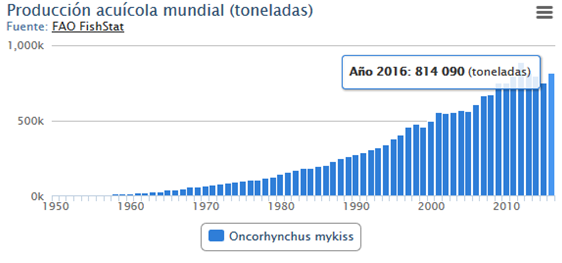
\includegraphics[width=1\textwidth]{introduction/produccion agricola mundial.png}
	%\caption{Ejemplo de imagen.}
	%\label{fig:PLACEHOLDER}
\end{figure}